% GNUPLOT: LaTeX picture with Postscript
\begingroup
  \makeatletter
  \providecommand\color[2][]{%
    \GenericError{(gnuplot) \space\space\space\@spaces}{%
      Package color not loaded in conjunction with
      terminal option `colourtext'%
    }{See the gnuplot documentation for explanation.%
    }{Either use 'blacktext' in gnuplot or load the package
      color.sty in LaTeX.}%
    \renewcommand\color[2][]{}%
  }%
  \providecommand\includegraphics[2][]{%
    \GenericError{(gnuplot) \space\space\space\@spaces}{%
      Package graphicx or graphics not loaded%
    }{See the gnuplot documentation for explanation.%
    }{The gnuplot epslatex terminal needs graphicx.sty or graphics.sty.}%
    \renewcommand\includegraphics[2][]{}%
  }%
  \providecommand\rotatebox[2]{#2}%
  \@ifundefined{ifGPcolor}{%
    \newif\ifGPcolor
    \GPcolortrue
  }{}%
  \@ifundefined{ifGPblacktext}{%
    \newif\ifGPblacktext
    \GPblacktexttrue
  }{}%
  % define a \g@addto@macro without @ in the name:
  \let\gplgaddtomacro\g@addto@macro
  % define empty templates for all commands taking text:
  \gdef\gplbacktext{}%
  \gdef\gplfronttext{}%
  \makeatother
  \ifGPblacktext
    % no textcolor at all
    \def\colorrgb#1{}%
    \def\colorgray#1{}%
  \else
    % gray or color?
    \ifGPcolor
      \def\colorrgb#1{\color[rgb]{#1}}%
      \def\colorgray#1{\color[gray]{#1}}%
      \expandafter\def\csname LTw\endcsname{\color{white}}%
      \expandafter\def\csname LTb\endcsname{\color{black}}%
      \expandafter\def\csname LTa\endcsname{\color{black}}%
      \expandafter\def\csname LT0\endcsname{\color[rgb]{1,0,0}}%
      \expandafter\def\csname LT1\endcsname{\color[rgb]{0,1,0}}%
      \expandafter\def\csname LT2\endcsname{\color[rgb]{0,0,1}}%
      \expandafter\def\csname LT3\endcsname{\color[rgb]{1,0,1}}%
      \expandafter\def\csname LT4\endcsname{\color[rgb]{0,1,1}}%
      \expandafter\def\csname LT5\endcsname{\color[rgb]{1,1,0}}%
      \expandafter\def\csname LT6\endcsname{\color[rgb]{0,0,0}}%
      \expandafter\def\csname LT7\endcsname{\color[rgb]{1,0.3,0}}%
      \expandafter\def\csname LT8\endcsname{\color[rgb]{0.5,0.5,0.5}}%
    \else
      % gray
      \def\colorrgb#1{\color{black}}%
      \def\colorgray#1{\color[gray]{#1}}%
      \expandafter\def\csname LTw\endcsname{\color{white}}%
      \expandafter\def\csname LTb\endcsname{\color{black}}%
      \expandafter\def\csname LTa\endcsname{\color{black}}%
      \expandafter\def\csname LT0\endcsname{\color{black}}%
      \expandafter\def\csname LT1\endcsname{\color{black}}%
      \expandafter\def\csname LT2\endcsname{\color{black}}%
      \expandafter\def\csname LT3\endcsname{\color{black}}%
      \expandafter\def\csname LT4\endcsname{\color{black}}%
      \expandafter\def\csname LT5\endcsname{\color{black}}%
      \expandafter\def\csname LT6\endcsname{\color{black}}%
      \expandafter\def\csname LT7\endcsname{\color{black}}%
      \expandafter\def\csname LT8\endcsname{\color{black}}%
    \fi
  \fi
  \setlength{\unitlength}{0.0500bp}%
  \begin{picture}(8640.00,5760.00)%
    \gplgaddtomacro\gplbacktext{%
      \csname LTb\endcsname%
      \put(946,704){\makebox(0,0)[r]{\strut{} 0.5}}%
      \put(946,1388){\makebox(0,0)[r]{\strut{} 1}}%
      \put(946,2073){\makebox(0,0)[r]{\strut{} 1.5}}%
      \put(946,2757){\makebox(0,0)[r]{\strut{} 2}}%
      \put(946,3442){\makebox(0,0)[r]{\strut{} 2.5}}%
      \put(946,4126){\makebox(0,0)[r]{\strut{} 3}}%
      \put(946,4811){\makebox(0,0)[r]{\strut{} 3.5}}%
      \put(946,5495){\makebox(0,0)[r]{\strut{} 4}}%
      \put(1078,484){\makebox(0,0){\strut{} 0}}%
      \put(1795,484){\makebox(0,0){\strut{} 0.1}}%
      \put(2511,484){\makebox(0,0){\strut{} 0.2}}%
      \put(3228,484){\makebox(0,0){\strut{} 0.3}}%
      \put(3944,484){\makebox(0,0){\strut{} 0.4}}%
      \put(4661,484){\makebox(0,0){\strut{} 0.5}}%
      \put(5377,484){\makebox(0,0){\strut{} 0.6}}%
      \put(6094,484){\makebox(0,0){\strut{} 0.7}}%
      \put(6810,484){\makebox(0,0){\strut{} 0.8}}%
      \put(7526,484){\makebox(0,0){\strut{} 0.9}}%
      \put(8243,484){\makebox(0,0){\strut{} 1}}%
      \put(176,3099){\rotatebox{-270}{\makebox(0,0){\strut{}Probability density function}}}%
      \put(4660,154){\makebox(0,0){\strut{}$|\va{\hat{l}}_i \cdot \va{\hat{x}}_i| \qquad \va{\hat{x}}_i = \va{\hat{T}}_i, \, \va{\hat{\omega}}, \, \va{\hat{b}} $}}%
    }%
    \gplgaddtomacro\gplfronttext{%
      \csname LTb\endcsname%
      \put(2065,5322){\makebox(0,0)[l]{\strut{}$|\va{\hat{l}} \cdot \va{\hat{T}}_1|$}}%
      \csname LTb\endcsname%
      \put(2065,5102){\makebox(0,0)[l]{\strut{}$|\va{\hat{l}} \cdot \va{\hat{T}}_2|$}}%
      \csname LTb\endcsname%
      \put(2065,4882){\makebox(0,0)[l]{\strut{}$|\va{\hat{l}} \cdot \va{\hat{\omega}}|$}}%
      \csname LTb\endcsname%
      \put(2065,4662){\makebox(0,0)[l]{\strut{}$|\va{\hat{l}} \cdot \va{\hat{b}}|$}}%
    }%
    \gplbacktext
    \put(0,0){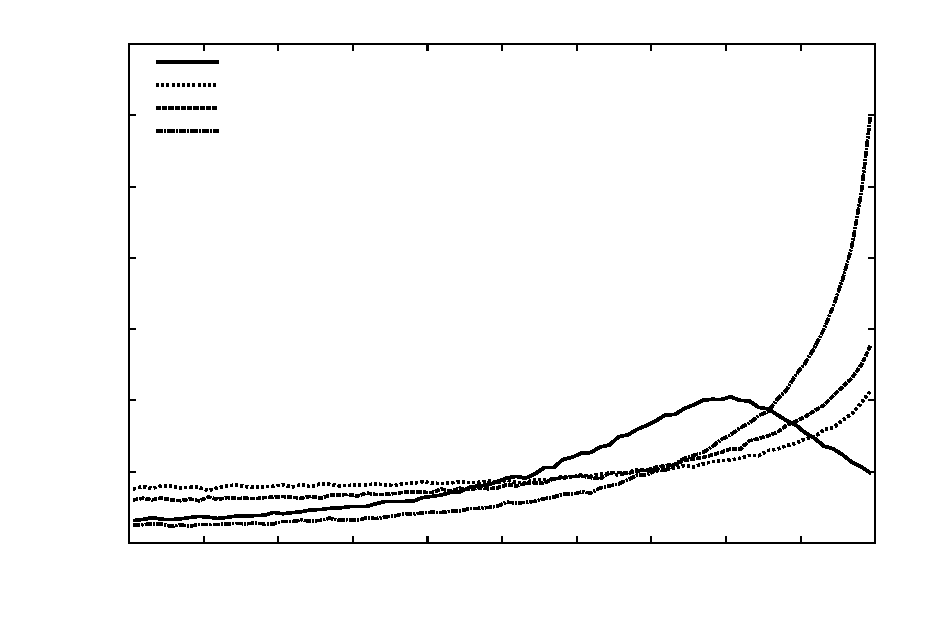
\includegraphics{figures/histograms/mhd_angle_histo_t20_Y00}}%
    \gplfronttext
  \end{picture}%
\endgroup
